\documentclass{report}

\usepackage{graphicx}
\usepackage{hyperref}
\usepackage{nth}
\usepackage{amsmath}
\usepackage{longtable}
\usepackage[margin=0.75in]{geometry}

\graphicspath{{./assets/}}

\title{SER-210 Final: Design Report}
\author{Thomas Kwashnak}



\begin{document}
\maketitle

\tableofcontents
\newpage

\chapter{Introduction}

\section{About the App}
The app described in this report is an attempt at making an easy go-to chat app to communicate with team members when working on a Github account. It aims to provide quick and easy chat rooms for each repositoriy, while only requiring the user to have a Github account.

\section{Report Purpose}
The purpose of this report is to provide an outline of plans made for the creation of the app. This report contains the UI Design plans, System Design plans, as well as an overview on the production plan over 3 iterations.

\newpage
\section{User Stories}
\textit{Last Modified: 4/13/2022}
\begin{itemize}
    \item As a user, I can sign in with my GitHub account to sign into the app
    \item As a user, I can view a list of recent chat rooms to quickly get back to what I was working on
    \item As a user, I can tap a star on a chat room to pin it to the top of the list so I have easy access to chat rooms I want
    \item As a user, I can select a chat room to open it up
    \item As a user, I can type and send a message into the chat room to interact with the conversation
    \item As a user, I can see chat messages appear so I can keep up with the conversation
    \item As a user, I can share a chat so I can invite friends into the chat
    \item As a user, I can create a new chat room for a chatRepository that I own so I can coordinate with other contributors
    \item As a user, I can type \# to reference a pull request or issue so viewers can click and navigate to that pull request or issue
    \item As a user, I can leave a chat room so I am not cluttered with chats I don't participate in
    \item As a user, I can view the app info so I know the app version and other information regarding the app
    \item As a user, I can log out of my account so I can log into another account
    \item As a user, I can click a link to redirect to the chatRepository page from the chat info
\end{itemize}

\chapter{UI Design}

\newpage
\section{Navigation Map}
\begin{center}
    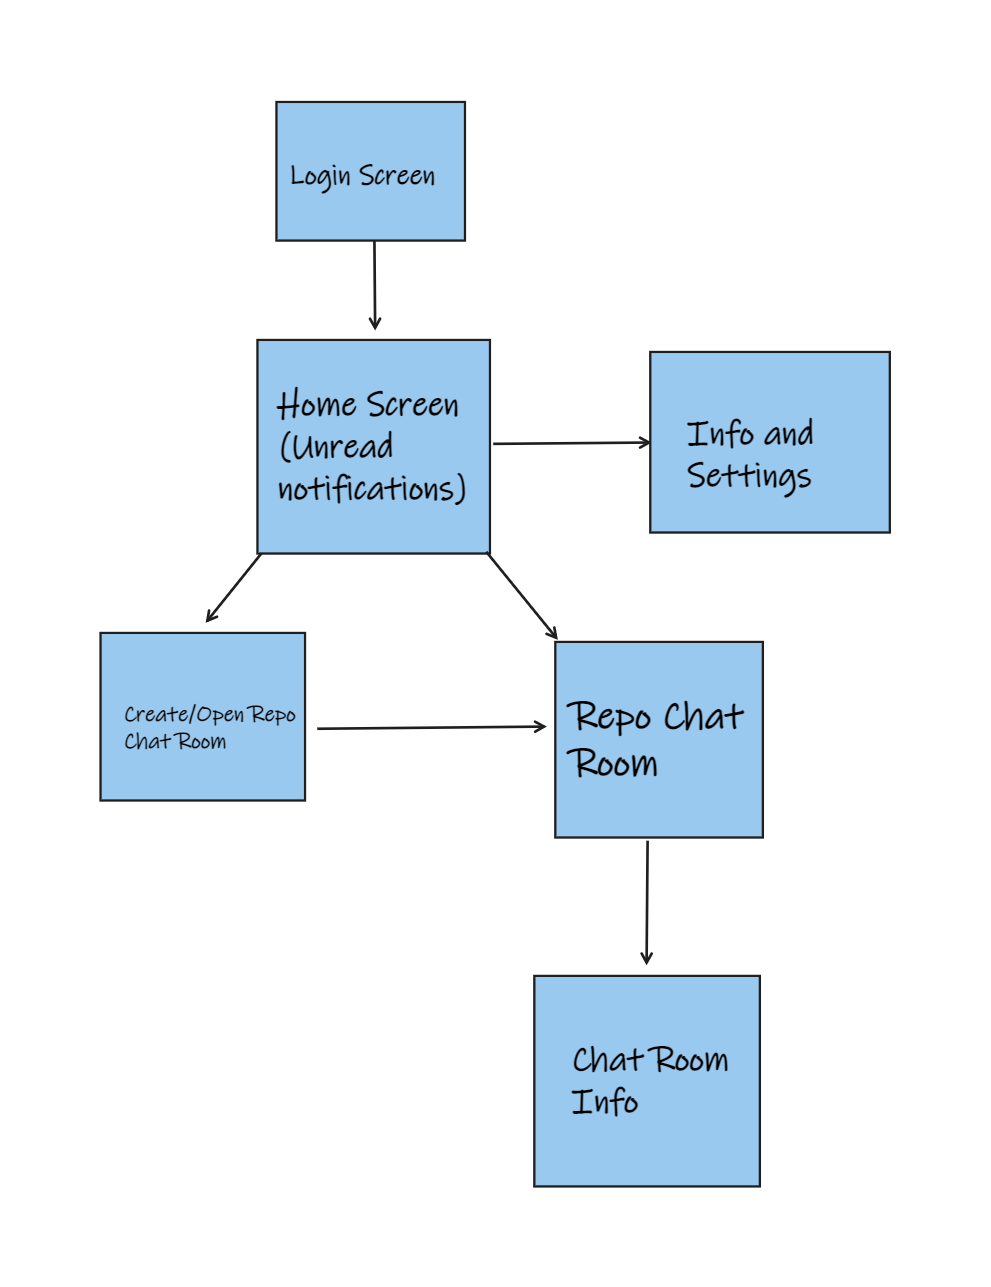
\includegraphics[width=\textwidth]{nav-graph}
\end{center}


\section{App Wireframes}

\subsection{Login Page}

\begin{center}
    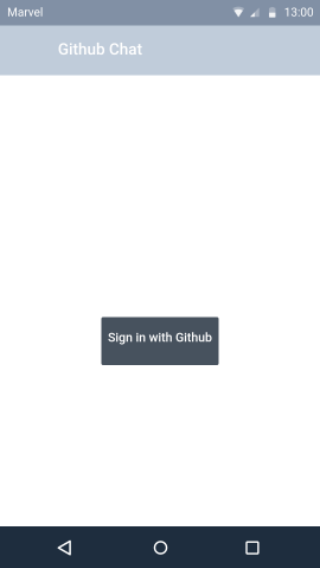
\includegraphics[scale=0.5]{design-login}
\end{center}
This is the landing page for the app after it first opens. If the user is signed in, then this page is bypassed. Otherwise, the user must sign in using their Github account.

\newpage
\subsection{Home Screen}

\begin{center}
    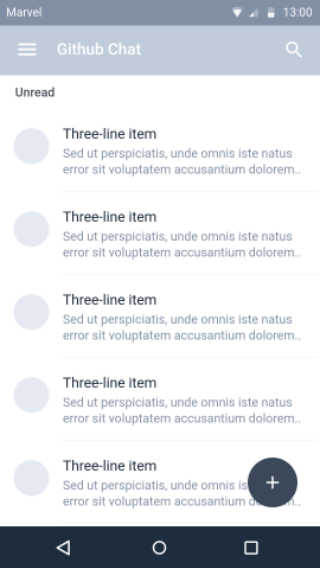
\includegraphics[scale=0.5]{design-home}
\end{center}

This is the home page. A list of recent repositories shows recent activity. A floating action button allows the user to create a new chat room for a repo. The user can select a "star" icon in order to "favorite" a chat

\newpage
\subsection{Navigation Drawer}

\begin{center}
    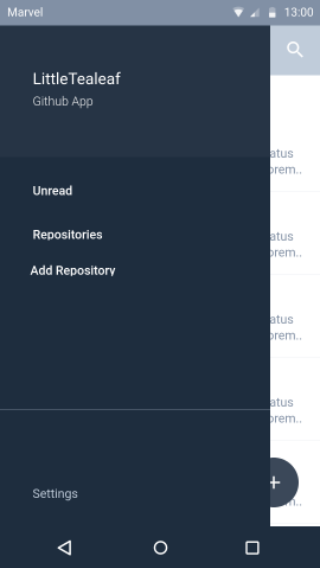
\includegraphics[scale=0.5]{design-nav-drawer}
\end{center}
The navigation drawer allows the user to access standard features such as adding repositories and opening settings


\newpage
\subsection{Options Screen}
\begin{center}
    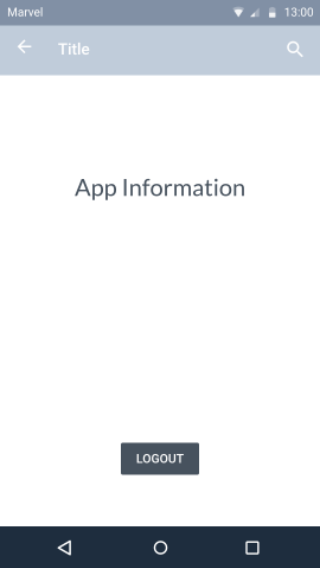
\includegraphics[scale=0.5]{design-options}
\end{center}
This screen displays the app information, and allows the user to log out of their account

\newpage
\subsection{Create Chat Screen}
\begin{center}
    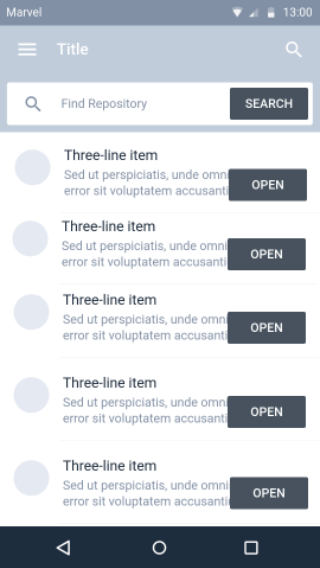
\includegraphics[scale=0.5]{design-create-chat}
\end{center}
This screen lists repositories the user owns, and the option to create a new chat room. The user can alternatively search up any chatRepository to create a chat room for that chatRepository.

\newpage
\subsection{Chat Screen}
\begin{center}
    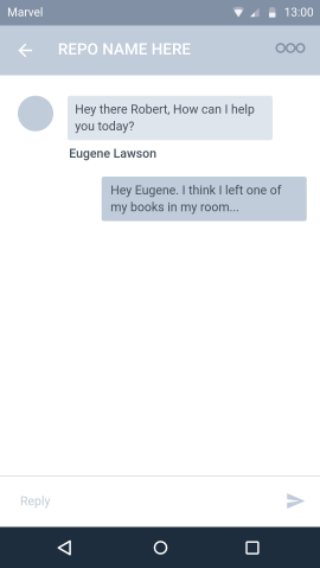
\includegraphics[scale=0.5]{design-chat}
\end{center}

This screen shows the actual chat room. The user can type a message into the message box. By typing \#, the user can link an issue or pull request.

\newpage
\subsection{Chat Info Screen}
\begin{center}
    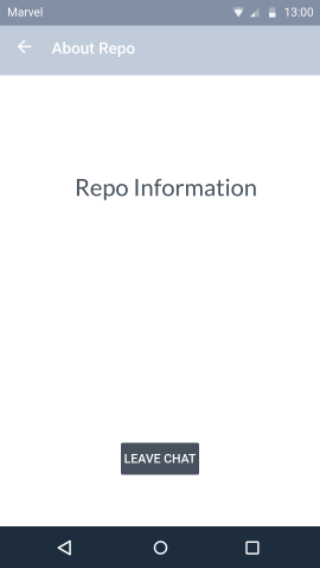
\includegraphics[scale=0.5]{design-chat-info}
\end{center}
This screen shows common chatRepository information, as well as a link the user can use to navigate to the chatRepository. Additionally, the user can click the leave chat to remove the chat from their list.

\newpage
\section{User Story Coverage}

\begin{center}
    \begin{tabular}{ | p{0.9\linewidth} |}
        \hline
        \textbf{Login Screen} \begin{itemize}
                                  \item As a user, I can sign in with my GitHub account to sign into the app
                              \end{itemize}                                                        \\
        \hline
        \textbf{Home Screen} \begin{itemize}
                                 \item As a user, I can view a list of recent chat rooms to quickly get back to what I was working on
                                 \item As a user, I can tap a star on a chat room to pin it ot the top of the list so I can keep chat rooms I want to keep on top
                                 \item As a user, I can select a chat room to open it up
                             \end{itemize}   \\
        \hline
        \textbf{Create Chat Screen}\begin{itemize}
                                       \item As a user, I can create a new chat room for a chatRepository that I own so I can coordinate with other contributors
                                   \end{itemize}        \\
        \hline
        \textbf{Chat Screen}\begin{itemize}
                                \item As a user, I can type and send a message into the chat room to interact with the conversation
                                \item As a user, I can see chat messages appear so I can keep up with the conversation
                                \item As a user, I can type \# to reference a pull request or issue so viewers can click and navigate to that pull request or issue

                            \end{itemize} \\
        \hline
        \textbf{Chat Info Screen}\begin{itemize}
                                     \item As a user, I can share a chat room so my friends can join
                                     \item As a user, I can click a link to redirect to the chatRepository page from the chat info
                                 \end{itemize}                                      \\
        \hline
        \textbf{Options Screen}\begin{itemize}
                                   \item As a user, I can log out of my account so I can log into another account
                                   \item As a user, I can view the app info so I know the app version and other information regarding the app

                               \end{itemize}                       \\
        \hline
    \end{tabular}
\end{center}

\chapter{System Design}

\section{Database Design}

\subsubsection{Messages}
\begin{tabular}{| l | l | l |}
    \hline
    \textbf{Name} & \textbf{Type} & \textbf{Key} \\
    \hline
    \hline
    \_id          & Integer       & Primary Key  \\
    \hline
    message       & String        & Not Null     \\
    \hline
    time          & Integer       & Not Null     \\
    \hline
    sender        & String        & Not Null     \\
    \hline
    apiSender     & Integer       & Foreign Key  \\
    \hline
    chatRepository    & Integer       & Foreign Key  \\
    \hline
    isRead        & Boolean       &              \\
    \hline
\end{tabular}
\subsubsection{Repositories (Chat Rooms)}
\begin{tabular}{| l | l | l |}
    \hline
    \textbf{Name} & \textbf{Type} & \textbf{Key} \\
    \hline
    \hline
    \_id          & Integer       & Primary Key  \\
    \hline
    name          & String        & Not Null     \\
    \hline
    apiRepo       & Integer       & Foreign Key  \\
    \hline
    apiPulls      & Integer       & Foreign Key  \\
    \hline
    apiIssues     & Integer       & Foreign Key  \\
    \hline
    isFavorite    & Boolean       &              \\
    \hline
\end{tabular}

\subsubsection{Github API Cache}
\begin{tabular}{| l | l | l |}
    \hline
    \textbf{Name} & \textbf{Type} & \textbf{Key} \\
    \hline
    \hline
    \_id          & Integer       & Primary Key  \\
    \hline
    url           & String        & Not Null     \\
    \hline
    content       & String        & Not Null     \\
    \hline
    fetchTime     & Integer       & Not Null     \\
    \hline
\end{tabular}

\section{Class Diagram}

\begin{center}
    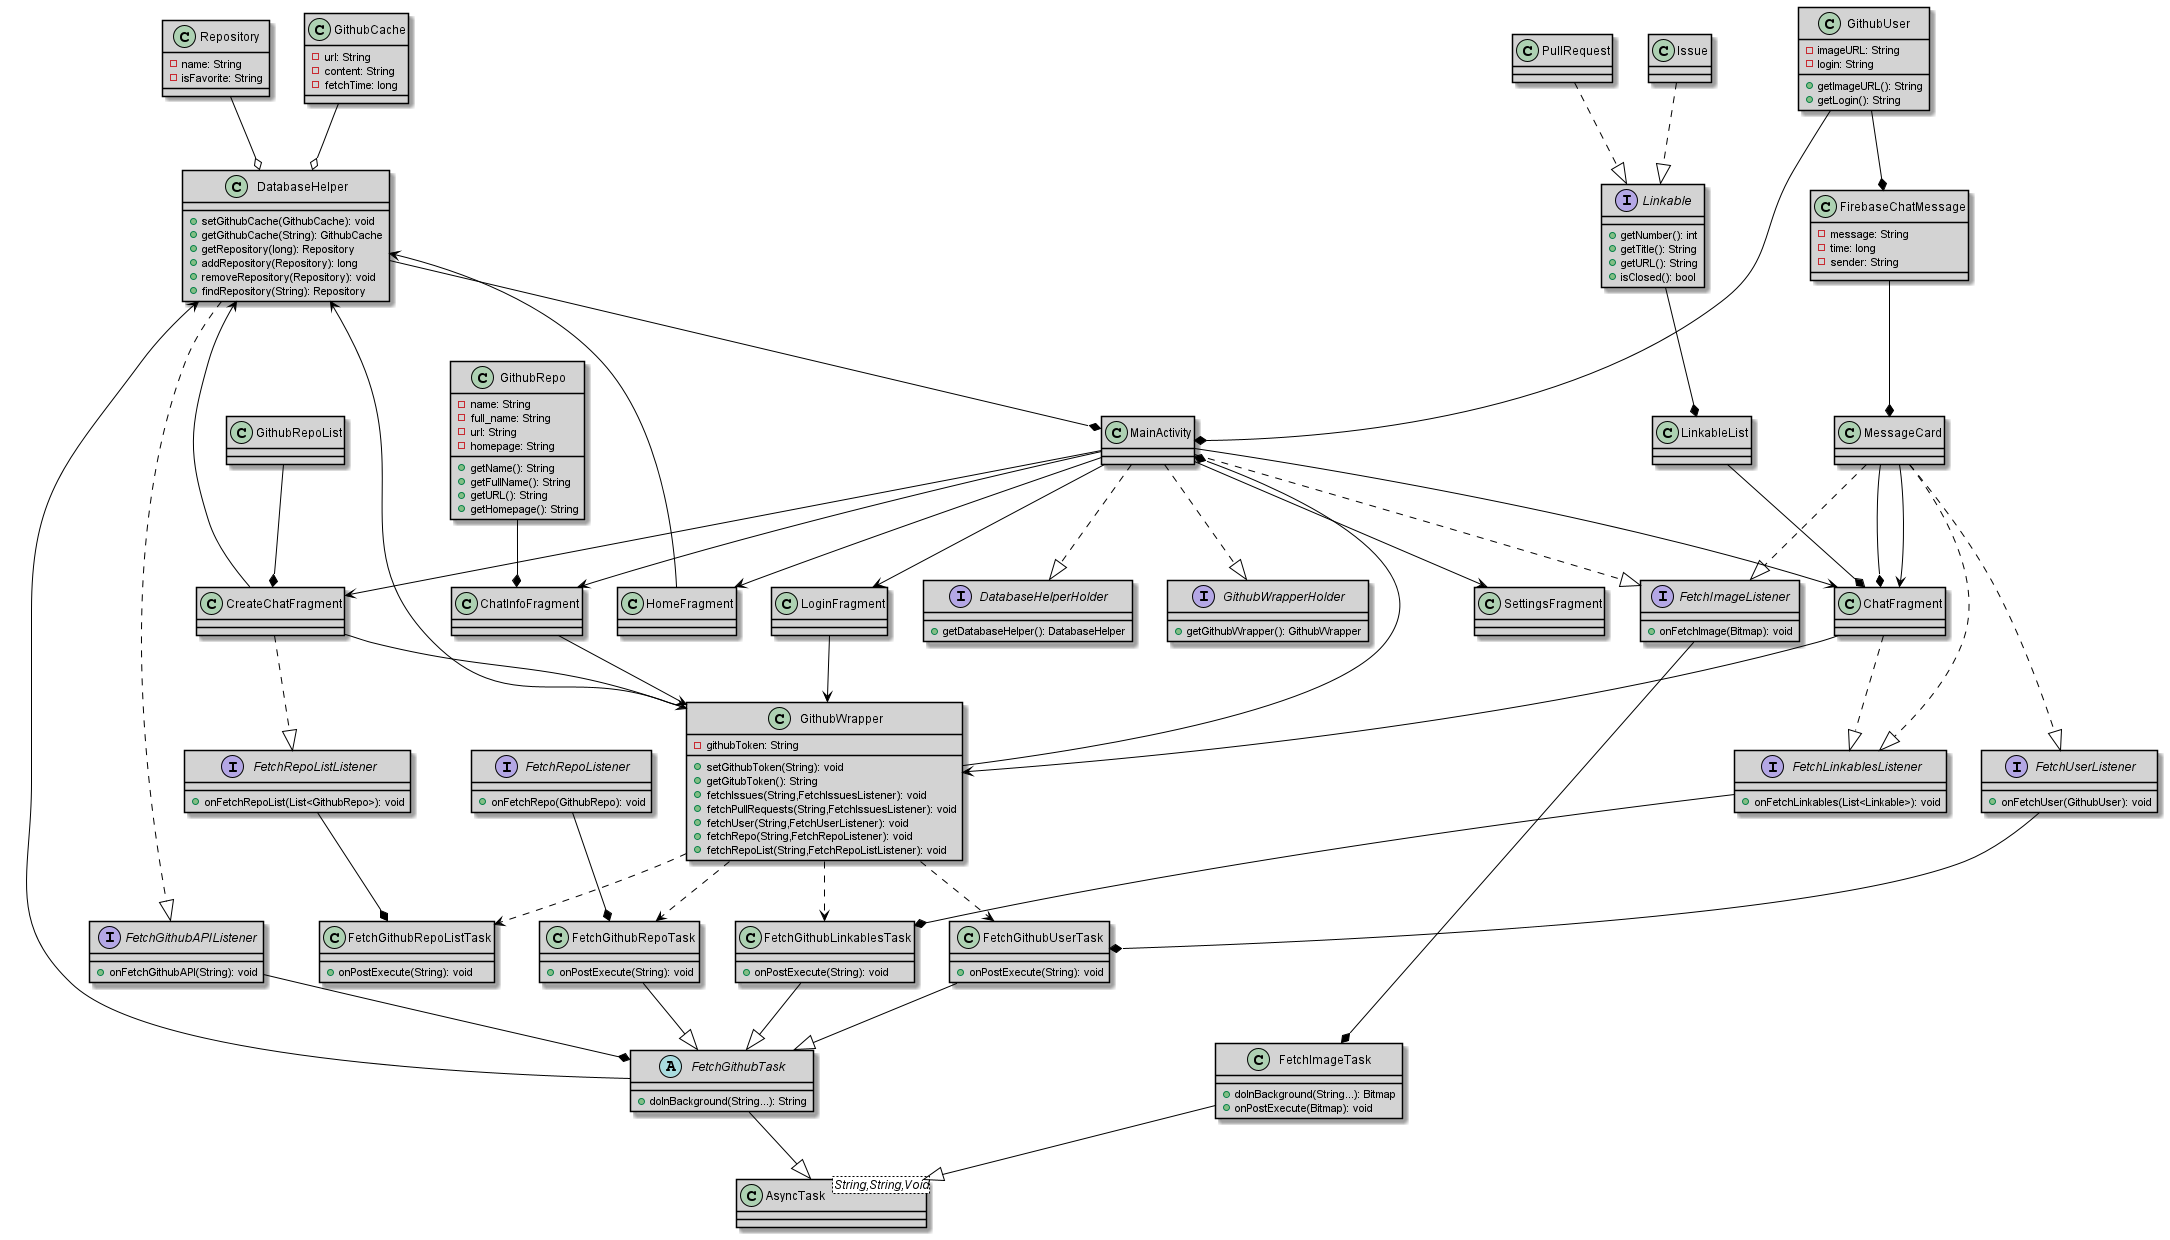
\includegraphics[scale=0.2]{class-diagram}
\end{center}
You can view the full diagram at \href{https://github.com/LittleTealeaf/SER-210-Final/blob/main/docs/reports/design/assets/class-diagram.png}{https://github.com/LittleTealeaf/SER-210-Final/blob/main/docs/reports/design/assets/class-diagram.png}\\

The class diagram is my current understanding of how the classes will be set up. In terms of the back-end, the Repository, GithubCache, and Message repositories are all generated directly from the LocalDatabase (I'll probably come up with a better name by then). The local database supports adding and retrieving Repositories, Messages, and Github Caches. The local database also supports updating GithubCaches with fresh values, which uses an interface to support the async task.

\section{Class User Stories}

\begin{center}
    \begin{tabular}{ | p{0.9\linewidth} |}
    \hline
    \textbf{LoginFragment} \begin{itemize}
                               \item As a user, I can sign in with my GitHub account to sign into the app
                           \end{itemize}                                                       \\
    \hline
    \textbf{ChatFragment} \begin{itemize}
                              \item I can view a list of recent chat rooms to quickly get back to what I was working on
                              \item As a user, I can type and send a message into the chat room to interact with the conversation
                              \item As a user, I can see chat messages appear so I can keep up with the conversation
                              \item I can tap a star on a chat room to pin it to the top of the list so I have easy access to chat rooms I want
                              \item As a user, I can share a chat so I can invite friends into the chat
                          \end{itemize}                 \\
    \hline
    \textbf{ChatInfoFragment} \begin{itemize}
                                  \item As a user, I can click a link to redirect to the chatRepository page from the chat info
                                  \item As a user, I can leave a chat room so I am not cluttered with chats I don't participate in
                              \end{itemize}                                     \\
    \hline
    \textbf{AppInfoFragment} \begin{itemize}
                                 \item As a user, I can view the app info so I know the app version and other information regarding the app
                             \end{itemize}                     \\
    \hline
    \textbf{Repository} \begin{itemize}
                            \item As a user, I can type \# to reference a pull request or issue so viewers can click and navigate to that pull request or issue
                        \end{itemize} \\
    \hline
    \textbf{CreateChatFragment} \begin{itemize}
                                    \item As a user, I can create a new chat room for a chatRepository that I own so I can coordinate with other contributors
                                \end{itemize}       \\
    \hline
    \textbf{HomeFragment} \begin{itemize}
                              \item As a user, I can view a list of recent chat rooms to quickly get back to what I was working on
                              \item As a user, I can select a chat room to open it up
                          \end{itemize}                              \\
    \hline
    \textbf{AppInfoFragment} \begin{itemize}
            \item As a user, I can log out of my account so I can log into another account
    \end{itemize} \\
    \hline
    \end{tabular}
\end{center}
\newpage

\chapter{Iteration Planning}

\section{Overall Iteration Plans}

The following are my goals for each iteration:

\subsection{Iteration 1}

The goal for this iteration is to get things initially set up. I will be focusing my efforts towards learning Firebase (and quickly falling back to a self-hosted server concept in case of catastrophic failure with Firebase), as well as getting the back end of the app intact.

By the end of the first iteration, I should have a very bare-bones app that allows you to log into your GitHub account, and then allows sending and, (hopefully) receiving  of messages

\subsection{Iteration 2}

The focus of this iteration is to take what I have from the last iteration and compartmentalize it into Chat rooms. The hope is that by the end of this iteartion, the app will have the ability to switch between chats, as well as creating chats from repositories.

\subsection{Iteration 3}

This iteration is the final "wrap everything up" iteration. That being said, many of the smaller and non-significant tasks are put into this last few weeks. Additionally, anything that I was unable to get done in previous weeks, or issues that I ran into, can be done during this iteration.

While I don't \textit{plan} on having much, if any, delaying of task completions across iterations, I do want to plan that time in so I don't get completely swamped by the 3rd iteration.

\section{Prioritized User Stories and Tasks}

User stories below are sorted from most to least prioritized. Times are ballpark, and most tasks will likely "merge" together as they are closely related.

\begin{enumerate}
    \item \textbf{Iteration 1}: (Additional Tasks)
    \item[] \begin{itemize}
        \item Set up Database Structure (\textbf{2 hours})
        \item Get GithubCache working properly (\textbf{1 hour})
    \end{itemize}
    \item \textbf{Iteration 1}: As a user, I can sign in with my GitHub account to sign into the app
    \item[] \begin{itemize}
        \item Set up and familiarize with Firebase (\textbf{1 hour})
        \item Enable authentication with Firebase (\textbf{1 hour})
        \item Integrate Authentication with Firebase into Application (\textbf{2 hours})
        \item Obtain usable Github API Token from from logging in (\textbf{2 hours})
    \end{itemize}
    \item \textbf{Iteration 1}: As a user, I can type and send a message into the chat room to interact with the conversation
    \item[] \begin{itemize}
        \item Figure out how storage works on Firebase (\textbf{1 hour})
        \item Create Mock-UI for sending/receiving  messages (\textbf{1 hour})
        \item Get app to send messages with proper values to Firebase (\textbf{2 hours})
        \item If all else fails, local-server the whole thing (Current backup thoughts is REST API server on localhost) (\textbf{3-7 optional hours})
    \end{itemize}
    \item \textbf{Iteration 1}: As a user, I can see chat messages appear so I can keep up with the conversation
    \item[] \textit{This very closely relates to the previous user story}
    \item[] \begin{itemize}
        \item Figure out how Firebase works with pulling data (\textbf{1 hour})
        \item Get App to display chat messages quickly after they appear on Firebase (\textbf{1 hour})
    \end{itemize}
    \item \textbf{Iteration 2}: As a user, I can create a new chat room for a chatRepository that I own so I can coordinate with other contributors
    \item[] \begin{itemize}
        \item Integrate fetching of user repositories (\textbf{1 hour})
        \item Create fragment to display user repositories (\textbf{2 hours})
        \item Implement ability to add a chatRepository to the database (\textbf{1 hour})
        \item Implement ability to manually add a chatRepository, as well as checking that the chatRepository exists (\textbf{2 hours})
    \end{itemize}

    \item \textbf{Iteration 2}: As a user, I can view a list of recent chat rooms to quickly get back to what I was working on
    \item[] \begin{itemize}
        \item Create fragment and display of open chat rooms (\textbf{2 hours})
        \item Set up custom ordering of chat rooms (\textbf{1 hour})
    \end{itemize}
    \item \textbf{Iteration 2}: As a user, I can select a chat room to open it up
    \item[] \begin{itemize}
        \item Create fragment to display chat messages (\textbf{2 hours})
        \item Add ability for fragment to send and receive messages (\textbf{3 hours})
    \end{itemize}
    \item \textbf{Iteration 2}: As a user, I can type \# to reference a pull request or issue so viewers can click and navigate to that pull request or issue
    \item[] \begin{itemize}
        \item Integrate fetching of Pull Requests and Issues from API (\textbf{2 hours})
        \item Create an "indicator" showing the title of the linked chat message as you type(\textbf{3 hours})
        \item Add an additional display for messages when issues or pull requests are referenced (\textbf{2 hours})
    \end{itemize}
    \item \textbf{Iteration 3}: As a user, I can leave a chat room so I am not cluttered with chats I don't participate in
    \item[] \begin{itemize}
        \item Create script to remove all messages and information for a single chatRepository (\textbf{1 hour})
        \item Add button providing the ability to leave a chat room (\textbf{1 hour})
    \end{itemize}
    \item \textbf{Iteration 3}: As a user, I can tap a star on a chat room to pin it to the top of the list so I have easy access to chat rooms I want
    \item[] \begin{itemize}
    \item Add ability to tap and "favorite" a chat room (\textbf{2 hours})
        \item Update sorting algorithm to prioritize starred chats (\textbf{1 hour})
    \end{itemize}
    \item \textbf{Iteration 3}: As a user, I can view the app info so I know the app version and other information regarding the app
    \item[] \begin{itemize}
        \item Create app info fragment (\textbf{1 hour})
        \item Add app info to to the app info fragment (\textbf{1 hour})
    \end{itemize}
    \item \textbf{Iteration 3}: As a user, I can click a link to redirect to the chatRepository page from the chat info
    \item[] \begin{itemize}
        \item Create link that redirects from the chat info fragment to the repo link (\textbf{1 hour})
    \end{itemize}
    \item \textbf{Iteration 3}: As a user, I can log out of my account so I can log into another account
    \item[]\begin{itemize}
        \item Allow logging out (\textbf{1 hour})
        \item Separate databases based on user login (\textbf{2 hours})
    \end{itemize}
    \item \textbf{Iteration 3}: As a user, I can share a chat so I can invite friends into the chat
    \item[] \begin{itemize}
        \item Allow user to share a chat using a link (\textbf{1 hour})
        \item Allow a user to join a chat using an invite link (\textbf{2 hours})
        \item Register the app to open up share links (\textbf{3 hours}) \textit{This is only if I have time and/or I am determined enough}
    \end{itemize}
\end{enumerate}

\newpage
\section{My Task Organization}
For this project, I will be using Github Issues and Github Projects to organize tasks, notes on specific tasks, and more.

You can see my github tasks at \href{https://github.com/LittleTealeaf/SER-210-Final/issues}{https://github.com/LittleTealeaf/SER-210-Final/issues}

You can view the milestones indicated at \href{https://github.com/LittleTealeaf/SER-210-Final/milestones}{https://github.com/LittleTealeaf/SER-210-Final/milestones}

You can also see the project in table format at \href{https://github.com/users/LittleTealeaf/projects/3}{https://github.com/users/LittleTealeaf/projects/3}

\end{document}
